% simulant — Supplementary Material (2026-10-14 분리).
% 본문이 14,297 단어로 JHM Research Paper 통상 범위의 두 배였다. 패널 논증과
% 직접 맞물리지 않는 독성축·QSAR·탈동조·인 국소반응성을 여기로 옮긴다.
% 상호참조는 xr 로 건다. 빌드 순서는 build_paper.sh 가 고정한다.
\documentclass[11pt,a4paper]{article}
\usepackage[margin=2.4cm]{geometry}
\usepackage{times}
\usepackage{amsmath,amssymb,graphicx,booktabs}
\usepackage[hidelinks]{hyperref}
\usepackage{xr}
\externaldocument[M-]{main}
\renewcommand{\thesection}{S\arabic{section}}
\renewcommand{\thetable}{S\arabic{table}}
\renewcommand{\thefigure}{S\arabic{figure}}
\renewcommand{\arraystretch}{1.15}
\bibliographystyle{elsarticle-num}

\title{Supplementary Material\\[4pt]
\large Whether Chemical Warfare Agent Simulant Designations Look Supported
Depends on Which Compounds Are in the Comparison}
\author{Ku Kang \and Yoon Jeong Jang}
\date{}

\begin{document}
\maketitle

\noindent This Supplementary Material carries the acute toxicity axis, the
predictive interpolation of that axis, the decoupling test between fidelity and
toxicity, the phosphorus-local reactivity analysis, and the test of whether a
descriptor space corresponds to measured colorimetric array response. These results stand on
their own data and are referenced from the main text where they bear on it; they
are placed here because the argument of the main text turns on the composition
of the comparison panel and does not depend on them.

\subsection{Safety axis}
\label{meth:aegl}
Acute inhalation toxicity was taken as the EPA AEGL-3 value at 10~min,
the concentration above which life-threatening effects or death are predicted,
parsed directly from the official compiled table \cite{epaaegl2018}; the
derivation of these values for the agents is described by
Watson et al.~\cite{watson2006}, and the concentration--time exponent on which short-exposure
extrapolation of such criteria rests was established by ten Berge et al.~\cite{tenberge1986}.
A single fixed exposure duration was used rather than a derived
concentration--time surface, and the tier value is used directly as a
per-compound property rather than as an exceedance probability. Agent
degradation products, which carry their own and in places
distinct toxicity \cite{munro1999}, are outside the compound set. Values
published in ppm were converted using
$c\,[\mathrm{mg\,m^{-3}}] = c\,[\mathrm{ppm}] \times M / 24.45$. Compounds
without a value are recorded as such, with the reason, and are never imputed.

Extraction is the step on which every safety-axis number depends, so we describe
it in full. The compiled table carries 270 chemical entries that present an AEGL
table of their own, besides a holding list of substances for which the agency
states that values are not being developed. Reading a
ten-minute AEGL-3 from one of them is not simply a matter of taking the first
number on the AEGL-3 line, for four reasons that the table itself imposes. Some
entries place a footnote marker in the ten-minute cell and give the value below
the table, as \textit{AEGL 3 - 10 min = ** 40,000 ppm}, because the value exceeds
half the lower explosive limit. Some give values only for the shorter durations
and \textit{NR} for the longer ones, so the row carries three numbers rather than
five. Some print the agency's own mg~m$^{-3}$ equivalent beside each value, in
brackets for the agents and in parentheses elsewhere. And the text layer of the
document occasionally breaks one row across two lines. We therefore parse each
AEGL row into exactly five duration cells, where a cell is a number, an
\textit{NR}, a \textit{see below}, or a bare footnote marker, and refuse to use
any row that does not yield five; footnote lines are separated from table rows by
grammar before parsing, and the ten-minute value is read from the text following
the footnote's equals sign, so the duration labels that precede it cannot be
mistaken for values. Of the 270 entries, 261 yield a ten-minute AEGL-3: 252 from a table cell and
nine from a footnote. Two of those 261, magnesium aluminium phosphide and a 60\%
nonafluoroisobutyl ether preparation, carry no registry number in the table and
are set aside here, because without one their structure cannot be resolved
unambiguously, which leaves 259 (250 from a table cell and nine from a
footnote). They are not the two set aside in Section~\ref{sec:qsar}, which have
registry numbers but no single molecular structure.

Two independent checks were applied, and the distinction between them matters.
The conversion constant was checked against the agency's own bracketed
mg~m$^{-3}$ figures, which it reproduces to within 0.9--4.0\% over eight
comparisons (GB, GD, GA and GF at AEGL-2 and AEGL-3). That check validates the
arithmetic and nothing else: every agent value carrying a bracketed conversion is
below 1~ppm and contains no thousands separator, so a defect in numeric
extraction could not appear in it. The extraction itself was therefore checked
over the whole table by a second reader that shares neither the text-extraction
engine nor the algorithm: it renders the document with a different tool, locates
the character columns of the five duration labels in each header line, and reads
the ten-minute value from the corresponding substring of the AEGL-3 line. A
positional reader of this kind cannot reproduce a token-ordering fault, which is
the point of using one. The two readers agree on all 259 entries, on all 257 of
those that resolved to a structure and on all nineteen values in the
twenty-eight-compound panel, and the check covers all 25 values at or above
1000, where a thousands separator appears. We report the coverage of this check
and not only its pass rate, because a validation sample that excludes the failure
mode it is meant to detect establishes nothing.

\subsection{Predictive interpolation of the safety axis}
\label{sec:qsar}
To test whether the missing values could be filled, a random forest was trained
on $\log_{10}$(AEGL-3, 10~min) using 37 RDKit descriptors, with five random seeds,
five-fold cross-validation and 10\,000 bootstrap resamples for interval
estimates. Of the 259 entries with a ten-minute AEGL-3, 257 resolved to a
structure through PubChem; the two that did not are a mixed-isomer entry and a
protein toxin, neither of which has a single molecular structure. Five of the 257
are interhalogen compounds that RDKit cannot parse, and two were removed because
their stored structure failed the identity check described below, leaving 250.
Twenty of these are military chemical agents, identified by registry number
rather than by matching on name, and all twenty were held out of training and
used only for evaluation, leaving 230 for training. The held-out set is the G
series including cyclosarin, VX, sulfur mustard, the three nitrogen mustards,
lewisite~1, methyldichloroarsine, ethyldichloroarsine, phenyldichloroarsine,
diphenylchloroarsine, adamsite, BZ, phosgene oxime, hydrogen cyanide, phosgene
and chloropicrin. Matching on names rather than registry numbers is what makes
such a set hard to assemble: the table lists cyclosarin as ``GF Agent'', which a
pattern written for ``Agent G'' does not find, and it lists three arsenical
vesicants and BZ in rows whose longer durations are \textit{NR}, which a parser
that requires five numbers per row discards entirely. External validation on
held-out compounds rather than cross-validated statistics
alone is the minimum standard for a predictive structure--activity model
\cite{gramatica2007,tropsha2010}. An applicability domain was defined as the
mean distance to the five nearest training compounds in standardised descriptor
space, with the boundary at the 95th percentile of the training set's own such
distances. This is the $k$-nearest-neighbour distance criterion whose relation to
prediction accuracy was established by Sheridan et al.~\cite{sheridan2004} and which appears
among the standard formulations surveyed by Netzeva et al.~\cite{netzeva2005} and
Roy et al.~\cite{roy2015}; we have used the same construction to bound predictions in
hazard-prioritisation screens \cite{dbpcarto}. Whether such a domain can detect
a compound that is close in descriptor space but outside the training set's
mechanistic coverage is precisely what Section~\ref{res:qsar} tests, and is
related to the open-set problem of recognising an input as unfamiliar rather than
assigning it to a known class \cite{openset}.

\subsection{Decoupling test}
Candidates were the AEGL compounds for which structure, electronic descriptors
and a measured AEGL-3 were all available, excluding the authentic agents
themselves ($n=207$). Eight further records were set aside under four rules
declared in advance, all of which ask the same question: are these four
electronic descriptors defined for that species at all? A record is excluded if
its stored structure has more than one component, because the relative placement
of the fragments is arbitrary and the dipole moment is therefore undefined
(three records); if the species is open-shell, because
$\omega=\mu^{2}/2\eta$ is not defined in this form for such a species and the
orbital parse reads only one spin manifold (three); if it is a bare atom with no
bonds, because molecular descriptors carry no meaning (three); or if the
HOMO--LUMO gap is below 0.5~eV, because $\eta$ is half that gap and $\omega$
diverges as it approaches zero (one). Some records fall under more than one
rule. The gap rule is the one with a visible consequence: sodium cyanide returns
a gap of 0.097~eV and an $\omega$ of 1091~eV where the next smallest gap in the
pool is 1.31~eV, and because distances are computed on standardised descriptors
that single record compresses the $\omega$ axis for every other compound,
raising the pool standard deviation from 11.33 to 70.49. Retaining all eight
records changes the Spearman coefficient from $+0.004$ to $-0.022$ and leaves
every conclusion in Section~\ref{res:h1} unchanged. Fidelity was defined as the standardised
Euclidean distance in the four-dimensional electronic space to the nearest
authentic agent; safety as the measured $\log_{10}$(AEGL-3). For the quadrant analysis, the safety bar
was set at the measured AEGL-3 of dichloromethane, the incumbent
simulant, read from the parsed table rather than entered by hand; a replacement
simulant should not be more acutely toxic than the compound it replaces. Because
that bar turns out to be demanding, the count is also reported at one and two
orders of magnitude below it. Association was tested with Spearman and
Pearson correlation, with 10\,000-resample bootstrap confidence intervals
\cite{efron1986}. Effect sizes are reported with intervals rather than
$p$-values alone \cite{nakagawa2007}. Where a paired comparison was made,
normality of the paired differences was assessed by the Shapiro--Wilk test
\cite{shapiro1965} and the Wilcoxon signed-rank test \cite{wilcoxon1945} used
in place of a paired $t$-test where normality was rejected; those paired tests
are reported for completeness only, because, as Section~\ref{M-sec:perm} explains,
they are confounded by group size and the exact permutation test supersedes them.
Multiplicity is corrected within each panel configuration. The six distance
statistics applied to the three descriptor spaces form one family of eighteen
tests on the same descriptor table, and we report the whole family rather than a
selection from it, so the Benjamini-Hochberg procedure \cite{benjamini1995} is
applied across those eighteen and the smallest adjusted value is given in
Table~\ref{M-tab:ablation}. An earlier version of this work reported one nominal
value per space and declined to correct, on the ground that the spaces were
separate analyses. That ground fails once the statistic is also chosen by the
analyst, and we treat the earlier position as an error rather than a convention.

Defining that family is itself a choice, and a paper arguing that such choices
decide the answer cannot leave its own unexamined. We therefore report four
schemes rather than one. The eighteen tests are corrected together; the six
statistics are corrected within each space separately, treating the spaces as
three analyses; a single statistic, the mean difference, is treated as though it
had been specified in advance, leaving three tests; and, because the three
spaces are nested and the six statistics are functions of one distance matrix,
the dependence is handled exactly rather than approximated. All eighteen tests
are computed on the same enumeration of designations, so the joint null
distribution is available: for each designation we convert every test statistic
to its one-sided $p$ within its own null, take the smallest of the eighteen, and
read the observed smallest $p$ against that distribution. This is the
single-step min-$P$ procedure of Westfall and Young \cite{westfall1993}, and
because the permutations are shared it requires no assumption about the
correlation structure. We also report the approximation it replaces, the
effective number of independent tests estimated from the eigenvalues of the
correlation matrix of the eighteen nulls by the method of Li and Ji
\cite{liji2005} used as a Bonferroni divisor, so that the two can be compared.
The five answers are given in Table~\ref{M-tab:family} and they do not agree.

\subsection{Dimensionality and subspace controls}
\label{meth:dimdetail}
The structural and electronic spaces differ in dimension by more than an order of
magnitude, and the concentration of Euclidean distances depends on dimension, so
a difference between the two spaces is not by itself a difference between
chemistries. We bounded the effect in two ways, both reported in
Section~\ref{res:dimdetail}. The standardised structural space was truncated to its
first three principal components and the permutation test rerun on that
three-dimensional space. Separately, 500 random three-descriptor subsets of the
structural space were drawn without replacement (seed \texttt{0xC0DE}) and the
full exact permutation test run on each, giving the distribution of $p$ that an
arbitrary three-dimensional slice of these descriptors produces. The observed
structural value is interpretable only against that distribution.

The random-subspace control of Section~\ref{meth:dimdetail} draws three descriptors
from a correlated pool, so three descriptors do not carry three degrees of
freedom and the resulting rate of nominal significance may be inflated. We
repeated it on ZCA-whitened coordinates, obtained by standardising the
structural block, taking the eigendecomposition of its covariance, and applying
$V\Lambda^{-1/2}V^{\top}$ over the non-null eigenvalues, so that the coordinates
drawn from are uncorrelated by construction. Both the raw and the whitened rates
are reported. Draws were raised from 500 to 2000, which carries a Monte Carlo
standard error near one percentage point on a proportion and resolves a
percentile to 0.05.

\subsection{Measured colorimetric array response}
\label{meth:deltaE}
Measured response was taken from a 29-dye colorimetric array reported in earlier
work from this laboratory \cite{hazref,group3ref,ondeviceref}. Colour difference
$\Delta E$ is given per dye for three compound sets at nominal vapour
concentrations of 10, 50, 100 and 500 (arbitrary units as reported), in two
imaging channels: ultraviolet-excited emission and reflectance. The sets are
DMMP with GA, GB, GD, GF and VX; AC, CG, CK, HD, HN and L with PS; and four
A-series agents. The first two sets supply the twelve compounds that are also in the descriptor
panel: six of the six in the first set and six of the seven in the second, the
exception being nitrogen mustard HN, which the descriptor panel does not carry.
The third set is excluded entirely and the criterion is arithmetic rather than
editorial: none of its four compounds appears in the descriptor panel, so no
pair of a measured pattern and a descriptor distance can be formed from it. It
contributes to no analysis in this paper.

The three sets are different compounds measured on different plates, not
replicates, so no $\Delta E$ value is compared across sets; every analysis is run
within a set and the results are reported separately or combined only at the
level of correlation coefficients. The two channels are likewise not replicates
but physically different measurements, and the same compound's patterns in the
two channels agree only to a mean cosine of 0.584. They are therefore treated as
independent modalities, and agreement between them is used as evidence of
reproducibility rather than averaged away.

Each compound's 29-dimensional response at each concentration was scaled to unit
length, so that pattern rather than magnitude is compared. The compound-axis mean
was then subtracted at each concentration to remove the common non-negative
response component, and the resulting vectors were averaged over concentrations
and renormalised to give one pattern per compound per channel. Similarity is the
cosine between patterns and dissimilarity is one minus that. Confidence intervals
are bootstrapped over concentrations with 10\,000 resamples, which means they
describe variation across the four concentrations of one plate set and not
agreement between independent preparations.

Two properties of this processing constrain what the patterns can be used to
show, and we state both because the first version of this analysis did not.

Subtracting the compound-axis mean at each concentration makes the resulting
vectors sum to zero across compounds, which fixes the mean cosine between
distinct compounds at $-1/(n-1)$ for $n$ compounds in a set. A negative
between-compound cosine is therefore an identity of the centring and not
evidence that the array separates the compounds. We report the observed mean
against that floor in Section~\ref{res:arraydetail} rather than against zero.

Pairwise distances are not independent observations. A set of $n$ compounds
gives $\binom{n}{2}$ pairs that share compounds, so correlating measured
dissimilarity against descriptor distance over pairs and testing it as if the
pairs were independent inflates significance; the unit of analysis is the
compound. We therefore test the association by Mantel permutation
\cite{mantel1967}, permuting compound labels on the descriptor distance matrix
10\,000 times (seed \texttt{0xC0DE}) and comparing the observed Spearman
coefficient against $|\rho|$ of the permuted matrices. Both the Mantel value and
the value that treating pairs as independent would have given are reported, so
the size of the error is visible.

\subsection{Dimensionality and the value of the nominal result}
\label{res:dimdetail}

The structural space has 38 coordinates and the electronic space has 3. Euclidean
distance behaves differently in the two, so a difference between them could be
geometric rather than chemical. We tested that, and it is not. We also tested
what the nominal structural value is worth against the descriptors it was drawn
from, and there the answer is less comfortable.

Truncating the standardised structural space to its first three principal
components does not weaken the result; it strengthens it, from $p=0.028$ to
$p=0.0044$ on the twenty-eight-compound panel. At matched dimension the two
spaces are still 62-fold apart in $p$ (0.0044 against 0.275). Whatever separates
the structural from the electronic result, it is not that one space has more
coordinates than the other, and we say so because the opposite is the natural
suspicion and because an earlier draft of this paper entertained it.

The second control is the informative one. We drew 2000 random three-descriptor
subsets of the structural space and ran the full exact permutation test on each.
On the twenty-eight-compound panel the median $p$ is 0.094, the 5th to 95th
percentile range is 0.006 to 0.710, and 36.3\% of the subspaces reach $p<0.05$
(Monte Carlo standard error 1.08 percentage points). The observed
38-dimensional value of 0.028 sits at the 25.8th percentile of that
distribution, and the electronic value of 0.275 at the 77.9th. Both are ordinary
draws. The three-principal-component value of 0.0044 sits at the 2.1st
percentile, which is what the leading components of a space should do and is not
independent evidence.

That rate is partly an artifact of the descriptors themselves, and we report the
correction because it is larger than we expected. Three descriptors drawn from a
correlated pool do not carry three degrees of freedom. Repeating the control on
ZCA-whitened coordinates (Section~\ref{meth:dimdetail}), where the coordinates are
uncorrelated by construction, the rate falls from 36.3\% to 16.9\% and the
median $p$ rises from 0.094 to 0.295. The correlation structure of the
structural block therefore inflates the apparent ease of reaching nominal
significance by more than a factor of two. The comparison that the argument
rests on is the percentile rather than the rate, and that is unaffected: the
observed value is an ordinary draw from the subspaces that were available to be
chosen.

So the structural and electronic spaces do differ, and the difference is
chemical rather than geometric; what the data do not support is that the
difference says anything about the compounds that were designated. A value at
the 28th percentile of the subspaces one could have chosen, in a family of
eighteen tests whose smallest adjusted value is 0.159, on the smaller of two
defensible panels, is not an argument. Picking a space, a panel and a statistic
fixes the answer, and the practice this paper examines has never written down
which to pick.

\subsection{Weighting the two descriptor blocks equally}
\label{res:blockbalance}

The merged space puts 38 structural coordinates and 3 electronic ones into one
Euclidean distance. Standardising each descriptor equalises the variance per
coordinate, not per block, so the expected contribution is 38 against 3 and the
merged distance is in practice a structural distance. The main text says so; this
section quantifies it, because a reader is entitled to ask whether the merged
result is an artifact of that imbalance. A colleague who read a draft asked
exactly this.

We repeated the whole analysis on a distance that equalises the expected
contribution of the two blocks,
\begin{equation}
d_{\mathrm{bal}}^{2}=\frac{1}{n_{s}}\sum_{i=1}^{n_{s}}(\Delta z_{s,i})^{2}
 +\frac{1}{n_{e}}\sum_{j=1}^{n_{e}}(\Delta z_{e,j})^{2},
\end{equation}
with $n_{s}=38$ and $n_{e}=3$, leaving the structural and electronic spaces
untouched since each is a single block. The same exact enumeration was used, over
the same three configurations, with the same six statistics.

\begin{table}[!htb]
\centering
\caption{Equal weight per descriptor against equal weight per block, in the
merged space. Valid-match counts are identical under the two weightings. The
smallest $p$ is taken over the eighteen-test family of three spaces by six
statistics, and $q$ is the Benjamini--Hochberg adjusted value of that family.}
\label{tab:blockbalance}
\small
\begin{tabular}{lccccc}
\hline
 & Valid & \multicolumn{2}{c}{Smallest nominal $p$}
 & \multicolumn{2}{c}{Smallest $q$} \\
Configuration & matches & per descriptor & per block
 & per descriptor & per block \\
\hline
Thirty-five, incumbent three & 0/11 & 0.151 & 0.076 & 0.617 & 0.617 \\
Thirty-five, plus literature eight & 5/11 & 0.039 & 0.021 & 0.212 & 0.222 \\
Twenty-eight, incumbent three & 3/11 & 0.025 & 0.009 & 0.159 & 0.132 \\
\hline
\end{tabular}
\end{table}

Two things follow, and they point in opposite directions. The valid-match counts
do not move at all: zero of eleven on the primary panel, five with the literature
eight admitted, three on the twenty-eight-compound panel, exactly as reported in
the main text. The paper's headline is therefore invariant to the weighting, and
so is the pre-specified-statistic counterfactual of Table~\ref{M-tab:family},
which stays at 0.042 on the twenty-eight-compound panel: the merged nominal value
there falls from 0.025 to 0.015, but the value that binds after correction is the
structural one, which the reweighting does not touch. No configuration has a
Benjamini--Hochberg adjusted value below 0.05 under either weighting.

Every nominal $p$ falls, however, and that is why the main text states the
primary-panel result as a conclusion about significance rather than as a
numerical floor. The smallest value of the eighteen-test family there is 0.151
with equal weight per descriptor and 0.076 with equal weight per block, so a
floor quoted from either weighting would not hold under the other. The direction
is away from the designations: equalising the blocks makes the incumbent
simulants look better on the nominal scale while leaving them with no agent
matched. Block weighting is therefore a fourth choice of the same kind as the
panel, the space and the statistic, and it was not declared in advance either.
We report it because we did not pre-register it, and because a reader who did
would have obtained numbers we would not otherwise have published.

\subsection{What the test could have detected}
\label{res:mde}

A null result invites the question whether the design could have seen an effect
at all, and the exact enumeration answers it without further assumption. We
moved the incumbent simulants closer to the agents by $\delta$, measured in
typical nearest-neighbour separations of the same space, left the rest of the
panel untouched, and read the shifted statistic against the null built from the
unmodified distances. The reading is conditional: on this panel, with only the
designated three made more faithful, the test returns $p<0.05$ at
$\delta = 0.22$ (Figure~\ref{fig:mde}). At $\delta = 0$ it returns 0.2831 on
the primary panel and 0.0250 on the twenty-eight-compound panel, reproducing
Table~\ref{M-tab:ablation}.

The comparison that matters is between that value and the deficit the incumbent
compounds actually carry. Across the eleven agents the normalised difference
between the nearest incumbent simulant and the nearest other compound has a
median of 0.463, more than twice the detectable value. Only at sarin, where it
is 0.117, does it fall below what the test can resolve, and that is the agent at
which the descriptor bootstrap of Section~\ref{M-res:panels} is also weakest,
recovering DMMP as nearest in 37.8\% of replicates. The null on the primary
panel is therefore a statement about the data rather than about the sensitivity
of the design, with sarin the one case where the two cannot be separated.

\begin{figure}[!htb]
\centering
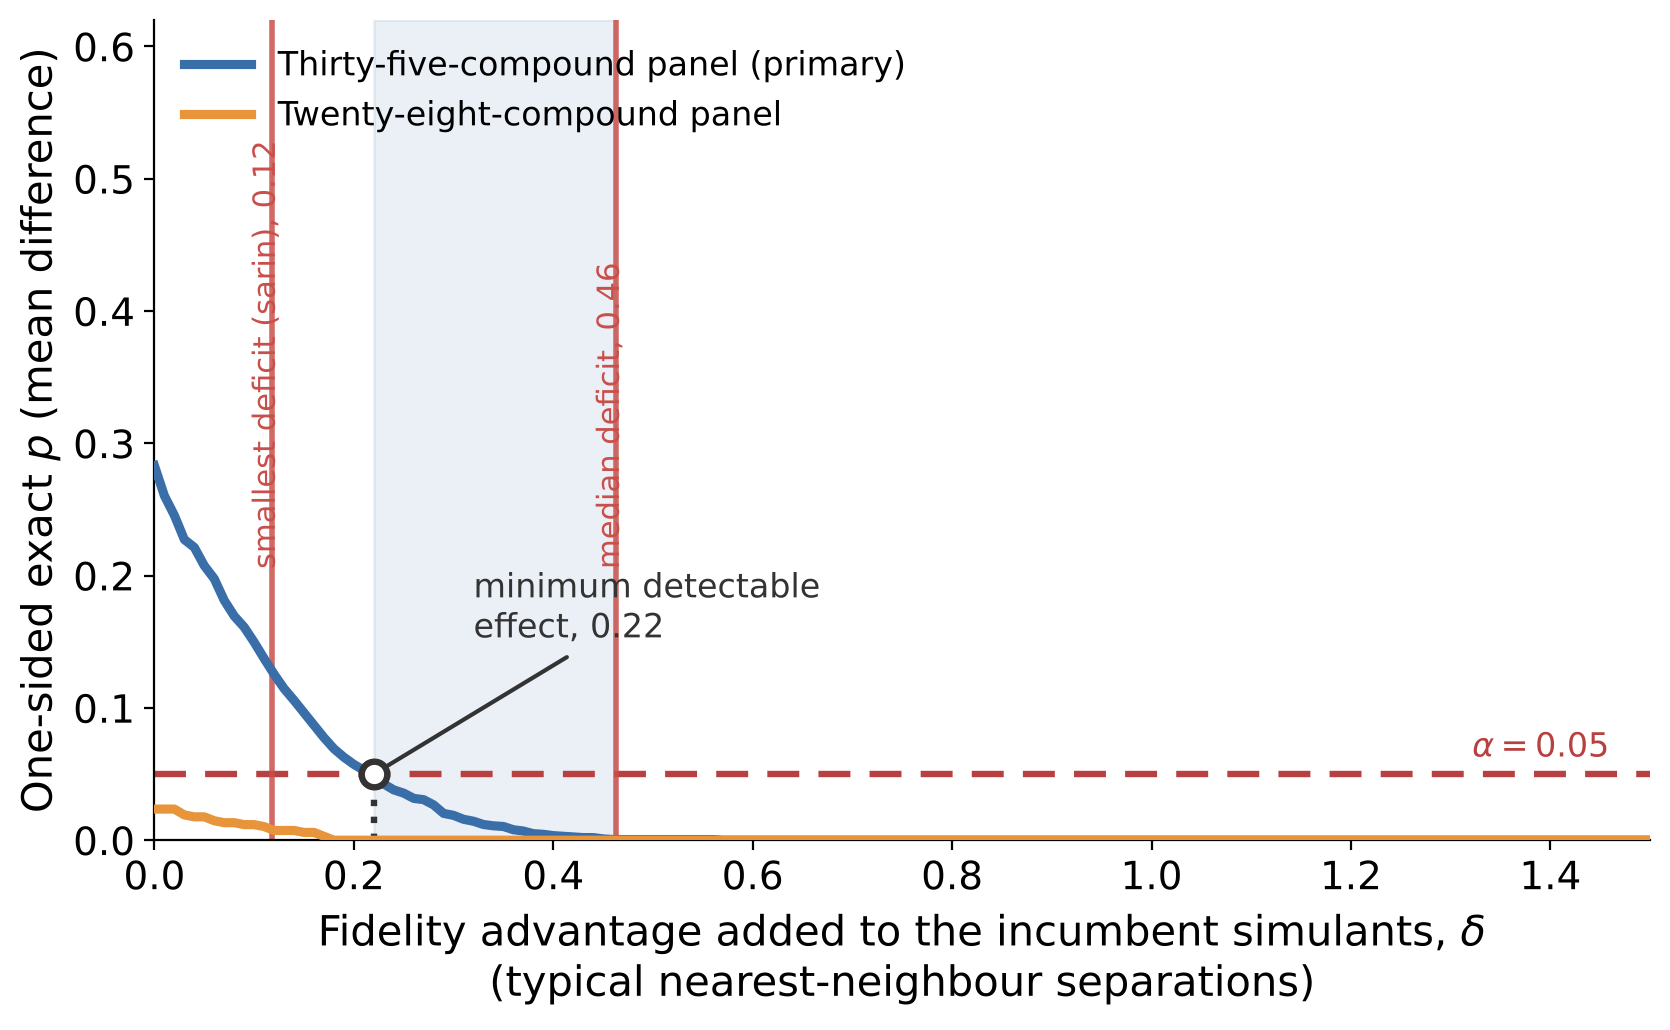
\includegraphics[width=\textwidth]{Fig_mde.png}
\caption{What the permutation test could have detected. One-sided exact $p$ for
the mean-difference statistic as the incumbent simulants are moved $\delta$
typical nearest-neighbour separations closer to the eleven agents, with the rest
of each panel unchanged and the null taken from the unmodified distances. On the
primary panel the test crosses $\alpha = 0.05$ at $\delta = 0.22$. The shaded
band spans that value and the median deficit the incumbent compounds actually
carry, 0.46; the deficit falls below the detectable value only at sarin.}
\label{fig:mde}
\end{figure}

\begin{figure}[t]
\centering
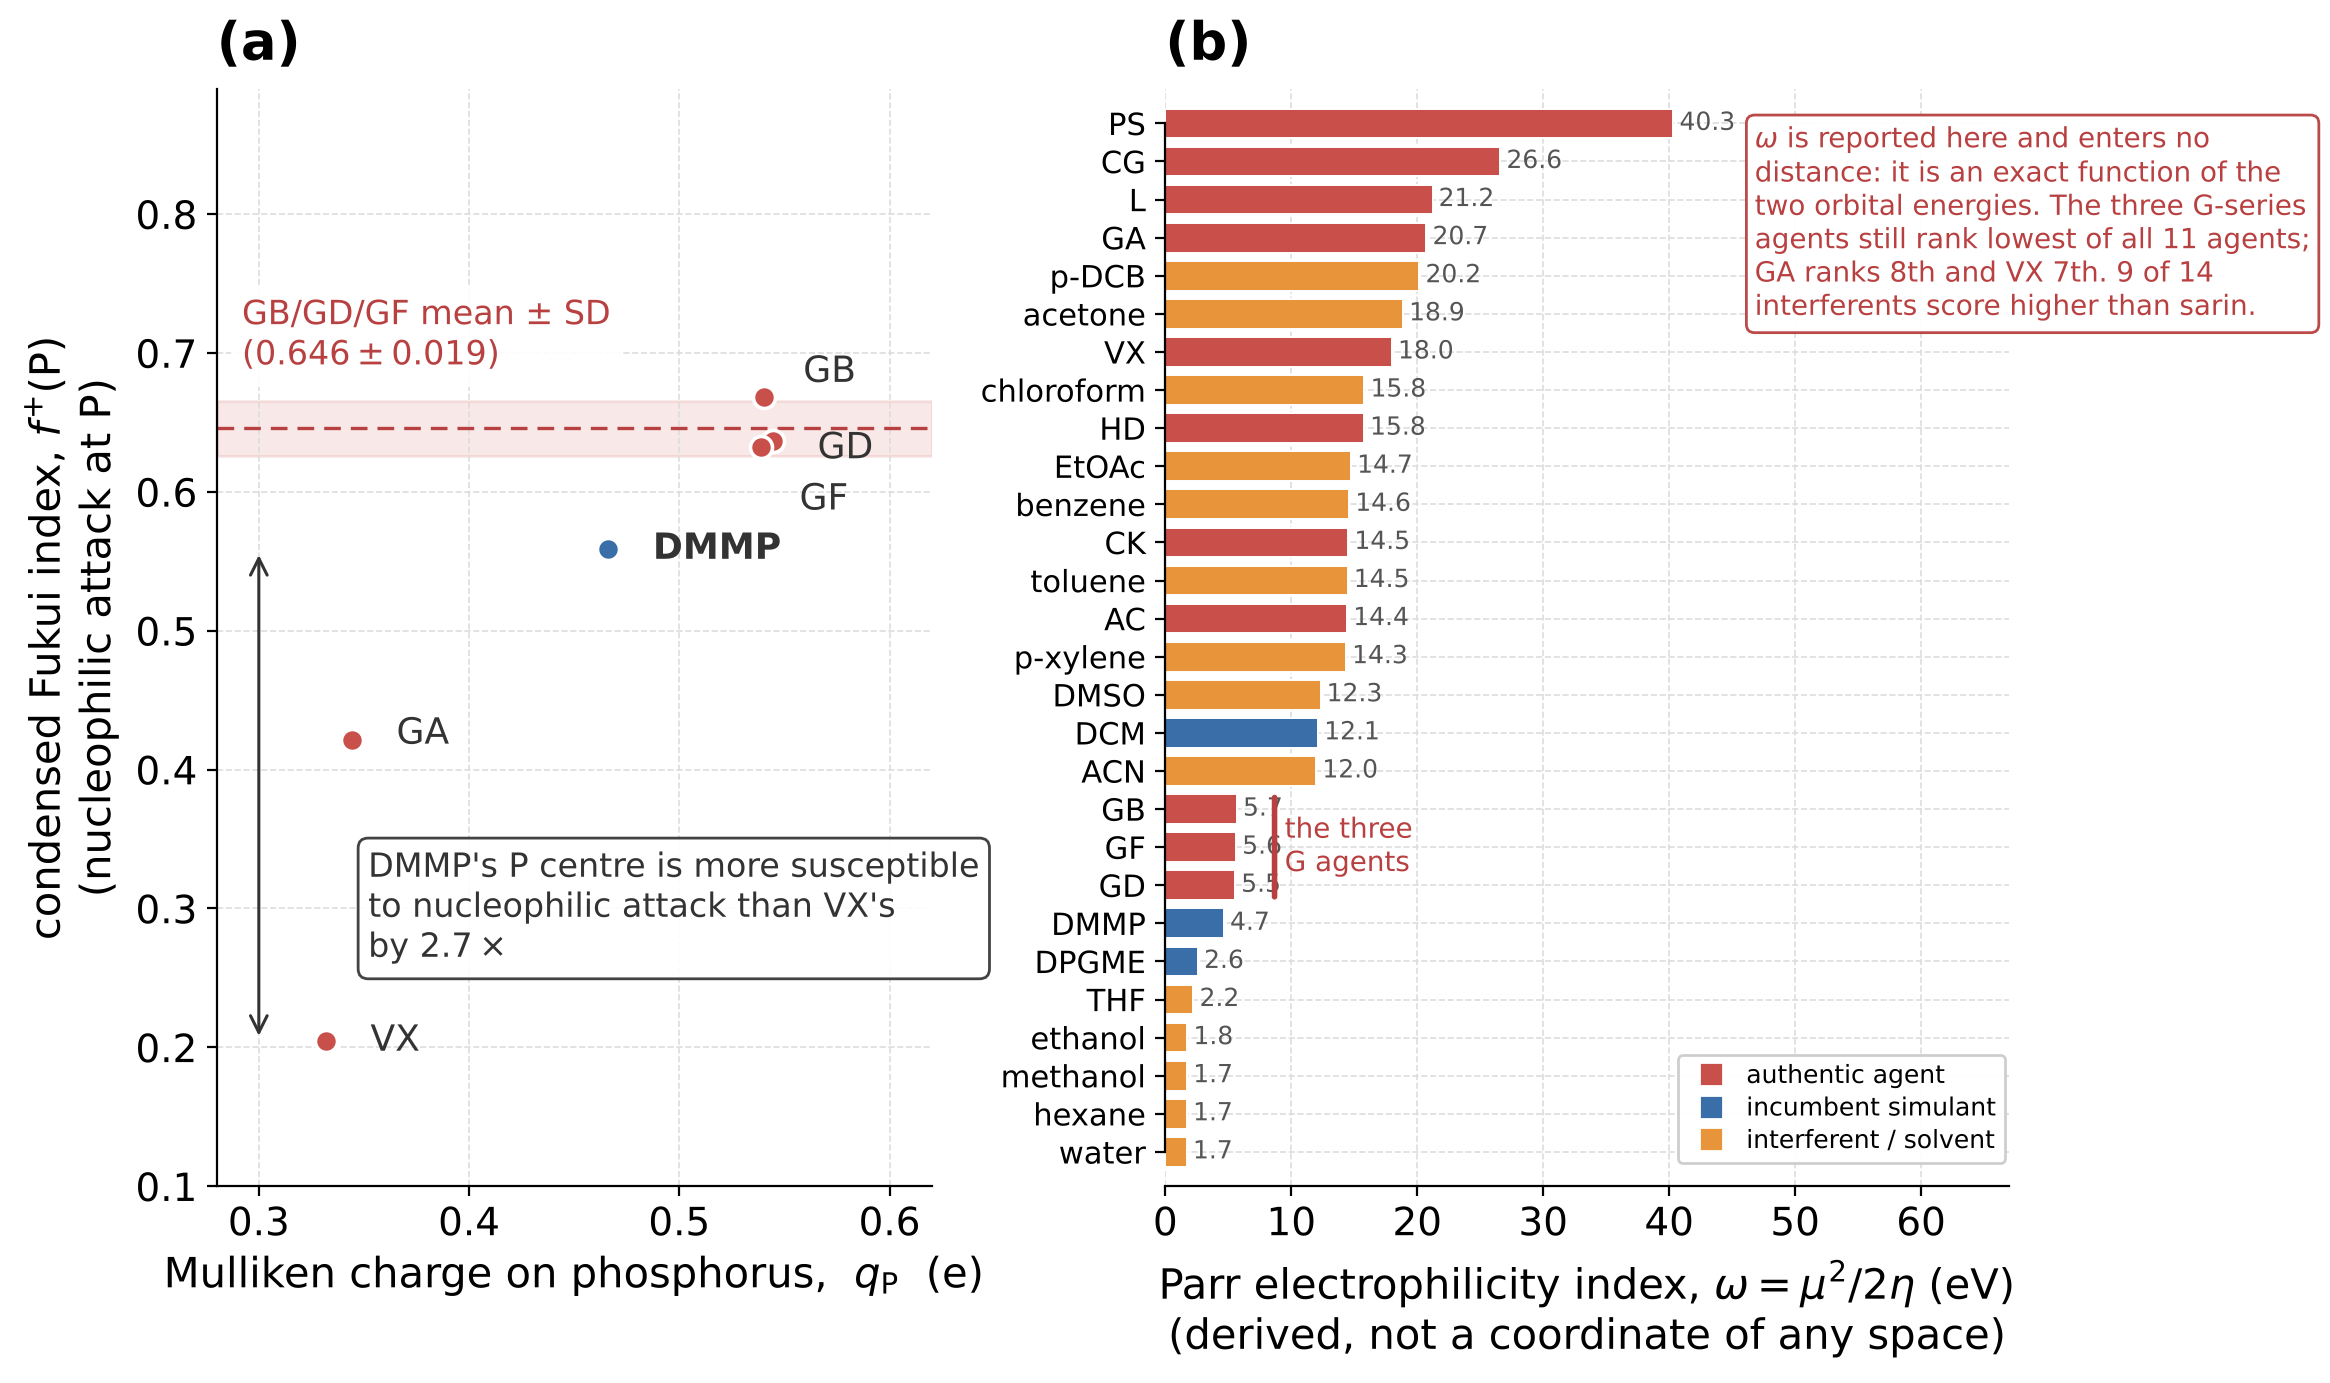
\includegraphics[width=\textwidth]{Fig_plocal.png}
\caption{Two quantities that sit outside every distance used in this work.
(a) Local electrophilicity against Mulliken charge at phosphorus for the six
phosphorus-bearing compounds (Section~\ref{res:plocal}). (b) The Parr
electrophilicity index, an exact function of the orbital energies that enter the
electronic space, which itself enters no distance anywhere in this work
(Section~\ref{M-meth:spaces}) and on which the three nerve agents rank lowest of
the eleven agents. The principal components of the two spaces are in
Figure~\ref{M-fig:spaces}a and b.}
\label{fig:plocal}
\end{figure}

\subsection{Local reactivity at phosphorus}
\label{res:plocal}

Table~\ref{tab:plocal} gives the phosphorus-centred quantities. The relevant
reactivity is the attack of the serine hydroxyl of acetylcholinesterase on
phosphorus, so the quantity of interest is the susceptibility of that centre to
a nucleophile, which is what $f^{+}(\mathrm{P})$ measures.

$f^{+}(\mathrm{P})$ orders GB $>$ GD $>$ GF $>$ DMMP $>$ GA $>$ VX. DMMP reaches
84\% of sarin's value but lies 4.47 standard deviations below the tight GB/GD/GF
cluster ($0.6456 \pm 0.0195$), so it is the closest available compound rather
than a member of the group. Against VX, DMMP's $f^{+}(\mathrm{P})$ is 2.73 times
larger.

That last ratio depends on which quantity is taken to represent local
reactivity, and we report both because they disagree. The composite local
electrophilicity of Domingo et al.~\cite{domingo2016},
$\omega_k = \omega f^{+}_k$, weights the condensed Fukui index by the global
index, and under it DMMP reaches 0.69 of sarin and 0.71 of VX rather than 2.73
times VX: the direction of the DMMP--VX comparison reverses. The reversal is
carried entirely by the global factor, which for VX is 17.99~eV because the
sulfur lone pair raises the HOMO, and for tabun 20.73~eV because of the nitrile.
Those are the same values that the next paragraph shows to be unusable as a
reactivity ordering for this compound class, so we do not treat $\omega_k$ as
the arbiter; but a reader applying the standard composite to Table~\ref{tab:plocal}
would reach the opposite conclusion about VX, and that is worth stating plainly.
Against the GB/GD/GF cluster the two conventions agree and $\omega_k$ is the
harsher of the two, placing DMMP 6.87 standard deviations below the cluster
against 4.47 for $f^{+}(\mathrm{P})$ alone.

The measured array response bears on this and narrows it.
Section~\ref{res:arraydetail} compares DMMP's 29-dye response pattern with those of
the authentic agents. DMMP is closer to sarin than to VX by 1.35 in cosine in
the ultraviolet channel and by 0.84 in reflectance, both intervals excluding
zero, so on the VX comparison the measurement sides with $f^{+}(\mathrm{P})$
against $\omega_k$. It does not support the wider reading that DMMP stands in
for the G series as a class: GD and GF are both further from DMMP than VX is.

\begin{table}[!htb]
\centering
\caption{GFN2-xTB local reactivity at phosphorus for the six phosphorus-bearing
compounds. $f^{+}(\mathrm{P})$ is the condensed Fukui index for nucleophilic
attack at phosphorus. $\omega$ is the global electrophilicity index in the
definition of Parr et al.~\cite{parr1999} with $\eta$ equal to half the
HOMO--LUMO gap, and $\omega_k = \omega f^{+}(\mathrm{P})$ is the composite local
electrophilicity of Domingo et al.~\cite{domingo2016}. The two reactivity
conventions disagree about VX and the text says why.}
\label{tab:plocal}
\small
\begin{tabular}{lcccccc}
\hline
Compound & $q_{\mathrm{P}}$ (e) & $q_{\mathrm{P=O}}$ (e) & $W_{\mathrm{P=O}}$ &
$f^{+}(\mathrm{P})$ & $\omega$ (eV) & $\omega_k$ (eV) \\
\hline
GB & 0.54044 & -0.42847 & 1.9527 & 0.66793 & 5.69 & 3.80 \\
GD & 0.54460 & -0.43006 & 1.9507 & 0.63692 & 5.54 & 3.53 \\
GF & 0.53868 & -0.42662 & 1.9546 & 0.63203 & 5.62 & 3.55 \\
\textbf{DMMP} & 0.46630 & -0.44588 & 1.9246 & 0.55852 & 4.66 & 2.60 \\
GA & 0.34433 & -0.38982 & 2.0146 & 0.42143 & 20.73 & 8.74 \\
VX & 0.33196 & -0.40303 & 1.9863 & 0.20431 & 17.99 & 3.68 \\
\hline
\multicolumn{7}{l}{\footnotesize GB/GD/GF mean $f^{+}(\mathrm{P})$ = 0.6456
$\pm$ 0.0195, DMMP 4.47 SD below; mean $\omega_k$ = 3.63 $\pm$ 0.15,}\\
\multicolumn{7}{l}{\footnotesize DMMP 6.87 SD below. $\omega$ and $\omega_k$ are
reported here and used in no distance (Section~\ref{M-meth:spaces}).}\\
\multicolumn{7}{l}{\footnotesize DMMP/VX = 2.73 by $f^{+}(\mathrm{P})$ but 0.71 by
$\omega_k$. Values are GFN2-derived and relative within one protocol.}\\
\end{tabular}
\end{table}

The Wiberg P=O bond order spans 1.9246--2.0146 across all six compounds and does
not separate the G series from DMMP; it carries no useful discrimination here.
The global electrophilicity index is actively misleading: GD (5.54), GF (5.62)
and GB (5.69) are the three lowest values among the eleven authentic agents, and
nine of the fourteen interferents score higher than sarin. The reason is that
$\omega$ responds to the lowest $\pi^{*}$ orbital wherever it sits, the nitrile
in tabun or the sulfur lone pair raising the HOMO in VX, and it has no particular
connection to phosphorus. Global electrophilicity should not be used as a
reactivity axis for this compound class.

\subsection{What the array actually measures}
\label{res:arraydetail}

Every argument above rests on descriptor distances, and the premise that one of
those spaces corresponds to what a vapour-phase sensor reports has so far been
assumed rather than shown. We test it against measured response from a
29-dye colorimetric array, reported for three compound sets at four
concentrations in two imaging channels, ultraviolet-excited and reflectance
(Section~\ref{meth:deltaE}). Twelve of the measured compounds are in the panel:
DMMP and the five nerve agents in the first set, and six of the remaining agents
in the second.

The array discriminates, but only after the common-mode response is removed, and
less of that separation is empirical than the raw numbers suggest. Colour
difference is a non-negative quantity, so every analyte shares a common
``something responded'' component and cosine similarity between raw profiles is
compressed towards unity. Between-compound similarity of 0.77 to 0.80 is not
separable from the within-compound value of 0.79 to 0.83 across concentrations
($p = 0.06$ to $0.94$). Subtracting the compound-axis mean at each concentration
separates them, to $+0.35$ to $+0.54$ within compounds against $-0.10$ to $-0.33$
between them, in all six combinations of compound set and channel ($p = 8 \times
10^{-5}$ to $0.025$).

The between-compound half of that contrast is largely arithmetic. Centring forces
the mean cosine between distinct compounds to $-1/(n-1)$, which is $-0.200$ for
the six-compound sets and $-0.167$ for the seven-compound set
(Section~\ref{meth:deltaE}). The observed means clear that floor by 0.013 to
0.066: $-0.187$ and $-0.167$ for the first set in the two channels against a
floor of $-0.200$, and $-0.101$ and $-0.117$ for the second against $-0.167$. The
negative between-compound similarity is therefore not evidence of separation. The
within-compound reproducibility across concentrations, which carries no such
constraint, is the part of this comparison that remains informative. All results
below use the centred patterns, with that caveat attached.

The measurement bears on Supplementary Section~\ref{res:plocal}, and it narrows the claim
rather than confirming it. What replicates across both channels is specific to
sarin. DMMP's pattern is closer to GB than to VX by 1.347 in cosine in the
ultraviolet channel (95\% CI 1.062 to 1.436, bootstrapped over concentrations)
and by 0.841 in reflectance (0.462 to 0.903), and closer to GB than to the mean
of GD, GF and VX by 1.284 and 0.984 in the two channels, every interval
excluding zero. The class-level statement is weaker. Taking the mean of the
three matched G agents against VX gives 0.513 (0.131 to 0.722) in the
ultraviolet channel but 0.137 (-0.144 to 0.290) in reflectance, and the least
similar agent to DMMP is GF rather than VX in both channels (-0.721 and -0.496
against -0.702 and -0.273 for VX).

The full ranking contains one result that the descriptor analysis does not
anticipate, and we give the whole ranking rather than the comparison we set out
to make. In the ultraviolet channel the agent nearest to DMMP is not sarin but
tabun, at $+0.764$ against sarin's $+0.645$, with soman, VX and cyclosarin
following at $-0.492$, $-0.702$ and $-0.721$. In reflectance sarin leads at
$+0.569$ and tabun falls to $-0.112$. Tabun is not a match to DMMP under the
descriptor criterion of Section~\ref{M-res:match}: its normalised distance is 2.03,
outside the threshold of 2. So the one measured channel in which the ordering is
clearest puts at the top an agent the descriptor analysis excludes, and the
agreement between the two channels on tabun is the worst of any agent in the set.
We report this as a disagreement between the descriptor table and the measurement
and not as a correction to either, because two channels on one plate set cannot
settle which is right.

The descriptor analysis assigns GB, GD and GF to DMMP. The array places sarin
first in one channel and tabun first in the other, and does not place GD or GF
closer to DMMP than VX in either. A sensor chemistry calibrated on DMMP is
therefore being shown something that behaves like one G agent at a time, not like
the G series, and the descriptor match for the other two does not survive contact
with the measured response.

It does not answer the larger question in either direction. Pattern
dissimilarity, taken as $1 - \cos$ and correlated against descriptor distance,
gives the same inconsistent picture as the permutation tests of
Section~\ref{M-res:panels}. Tested by Mantel permutation over compounds
(Section~\ref{meth:deltaE}), two of the eight panel-channel-space cells reach a
nominal $p<0.05$, and they favour different spaces: the structural space in the
second compound set's ultraviolet channel ($\rho = +0.539$, Mantel $p = 0.012$)
and the electronic space in the same set's reflectance channel ($\rho = +0.571$,
Mantel $p = 0.047$). The first compound set gives nothing in either space or
channel ($|\rho| \le 0.225$, Mantel $p \ge 0.22$). The eight cells are one
family, and we correct them as we correct the permutation tests of
Section~\ref{M-res:panels}: under Benjamini-Hochberg the smallest adjusted value is
0.098 and no cell reaches $q<0.05$. We state the nominal values as well because
two cells pointing at different descriptor spaces is itself the pattern worth
seeing, but neither cell is a result.

Treating the fifteen pairs as independent observations, which the first version
of this analysis did, moves these values by up to 0.026 and in both directions:
it would have reported the structural cell at $p = 0.038$ rather than 0.012 and
the electronic cell at $p = 0.026$ rather than 0.047. The error is not large here
because the sets are small, but it is the error that would grow with panel size,
and it runs toward significance in the cell with the larger coefficient.

Pooling the two compound sets by Fisher transformation, which is legitimate
because they are different compounds on different plates, the structural space
gives $\rho = +0.317$ (95\% CI $-0.072$ to $+0.622$) in the ultraviolet channel
and $+0.168$ ($-0.227$ to $+0.515$) in reflectance, while the electronic space
gives $-0.110$ ($-0.471$ to $+0.281$) and $+0.327$ ($-0.061$ to $+0.629$). Every
interval contains zero. The electronic space is the better predictor in one of
the four cells.

Six compounds per set bound how much that null can carry. At $\alpha = 0.05$ and
80\% power the design detects $|\rho| \ge 0.669$ from fifteen pairs and $0.492$
pooled, and the Mantel null is built from the $6!$ relabellings of six compounds,
so the smallest attainable one-sided $p$ is of order $10^{-3}$ and the resolution
is coarse. These data exclude a strong association between either descriptor
space and the measured response and nothing weaker. They do not show that the
electronic space governs sensor response, do not place it above the structural
space, and do not show it to be irrelevant. The claims in the rest of this paper
are written to that limit.

\subsection{The measured safety axis, and the holes in it}

Nineteen of the twenty-eight compounds have an AEGL-3 at 10~min
(Fig.~\ref{M-fig:tox}a). The ordering runs VX (0.0295~mg~m$^{-3}$), soman (0.365),
sarin (0.367), cyclosarin (0.391), tabun (0.729), sulfur mustard (3.84),
lewisite~1 (3.9), chloropicrin (13.4), phosgene (14.6), hydrogen cyanide (29.8),
acetonitrile (403), chloroform (19\,530), benzene (30\,990), p-xylene (31\,264),
toluene (37\,685), acetone (38\,007), dichloromethane (41\,685), n-hexane
(42\,296) and methanol (52\,420). The axis spans six orders of magnitude, and
the incumbent simulant dichloromethane sits at the safe end of it,
$1.4\times10^{6}$ times less acutely toxic than VX and 1400 times less toxic
than hydrogen cyanide. On this axis the incumbent simulant is not the weak link.

It is, however, not the safest thing on the panel. Methanol and n-hexane both
carry higher AEGL-3 values than dichloromethane, and neither is used as a
simulant for anything. The point is not that either should be: it is that the
safety axis cannot be what selected the incumbent, because two ordinary
laboratory solvents on the same panel score better on it. Against the 207 AEGL
compounds that carry both axes (Section~\ref{res:h1}) dichloromethane sits at
the 96th percentile of measured acute inhalation safety, with seven compounds
above it. Taking the incumbent as the bar a replacement must meet therefore sets
a demanding bar, and the consequences are worked through in
Section~\ref{res:h1}.

Nine compounds have no value, all nine because they are absent from the AEGL
list: DMMP, tetrahydrofuran, ethyl acetate, water, DPGME, ethanol, DMSO,
p-dichlorobenzene and cyanogen chloride. Cyanogen chloride is the one military
agent among them, and its absence is a recorded decision rather than an
oversight: it appears in the compiled table's holding list, where the agency
states that values are not being developed. DMMP's position is worth stating
precisely, because it is the compound
that carries all three valid matches found above. EPA's provisional
peer-reviewed assessment declined to derive an inhalation reference
concentration, recording that the data are insufficient, and derived no
inhalation unit risk; no acute inhalation LC$_{50}$ is cited; IRIS and HEAST
contain no RfD, RfC or cancer value. What exists is an oral provisional RfD of
0.06~mg~kg$^{-1}$~day$^{-1}$ carrying an uncertainty factor of 3000, and an oral
cancer slope factor of $1.7\times10^{-3}$ (mg~kg$^{-1}$~day$^{-1}$)$^{-1}$ based
on mononuclear cell leukaemia in male rats, with the evidence characterised as
suggestive \cite{epapprtv2006}. The inhalation safety of the field's principal
nerve-agent simulant has not been established; it has not been assessed. The two
incumbent simulants therefore sit at opposite ends of the evidence, not of the
hazard: for dichloromethane there is a regulator-derived value and it is
favourable, and for DMMP there is a regulator's recorded decision not to derive
one.

Cyclosarin carries its own entry in the compiled table under CAS 329-99-7, with
a ten-minute AEGL-3 of 0.053~ppm bracketed by the agency as 0.38~mg~m$^{-3}$;
our conversion from the published parts-per-million value gives
0.39~mg~m$^{-3}$, placing it between sarin and tabun. The entry is titled
\textit{GF Agent} rather than \textit{Agent GF}, which is why matching on
compound names rather than on registry numbers can miss it;
Section~\ref{meth:aegl} describes the CAS-keyed procedure used here.

\subsection{A QSAR cannot fill the gaps}
\label{res:qsar}

On the training distribution the model works. The random forest
(Fig.~\ref{M-fig:tox}c and d) reached $R^{2}=0.458 \pm 0.014$ and RMSE $0.935$ in
$\log_{10}$ units (95\% CI 0.830--1.020) against a training-mean baseline of
1.271 (1.175--1.365) and a logP-plus-molecular-weight linear baseline of 1.225.
The intervals for the model and the mean baseline do not overlap, and the
out-of-fold error over the whole training set is unbiased, averaging $+0.001$ log
units. Nothing in the cross-validated statistics would warn a user off.

On the twenty agents held out of training it failed, in one direction and without
exception. Every one was predicted safer than measured, by between 0.40 and 3.42
log units, a factor of 2.5 to 2600. Sarin was placed at 29~mg~m$^{-3}$ against a
measured 0.367 and VX at 2.4 against 0.0295, errors of 79-fold and 80-fold.
Fourteen of the twenty lie inside the applicability domain, so for those the
domain check raises no objection, and the worst of those fourteen is still wrong
by 2.68 log units, a factor of 482. DMMP's domain distance, 3.28, sits among the
agents' own, which is to say inside the region where the model is wrong by one to
two orders of magnitude, so its prediction is not used.

\begin{sloppypar}
The explanation is not that the mechanism is missing from the training set. We
checked, because that was our first hypothesis and it is wrong. Thirteen of the
230 training compounds carry an acetylcholinesterase-inhibiting pharmacophore,
identified by substructure rather than by name: ten organophosphorus esters
(phorate, phosphamidon, monocrotophos, dicrotophos, fenamiphos, parathion,
methyl parathion, methamidophos, dichlorvos, malathion) and three carbamate
esters (aldicarb, oxamyl, methomyl). The mechanism by which the nerve agents
kill, phosphylation of the serine hydroxyl of acetylcholinesterase and the
cholinergic crisis that follows \cite{bajgar2004,thiermann2013,worek2020},
is therefore represented, and one of
the thirteen, phorate at 0.22~mg~m$^{-3}$, is more acutely toxic than sarin. The
model sees the mechanism and still cannot place the agents.
\end{sloppypar}

What it cannot do is reach either extreme. Over the whole training set the
out-of-fold error is centred on zero, but in the most toxic decile
(the 23 compounds at or below 3.21~mg~m$^{-3}$) it averages $+1.41$ log units
and is positive for every single compound, while in the least toxic decile (the
23 at or above 8094~mg~m$^{-3}$) it averages $-1.13$ log units and is negative
for all but one. The same symmetry appears inside the anticholinesterase subset
taken on its own: phorate, the most toxic of the thirteen, is predicted 177 times
too safe, while malathion, the least toxic, is predicted 269 times too toxic.
This is regression toward the mean at both tails, which is what a
variance-minimising ensemble does with sparsely populated extremes, and the
agents are all in one of them.

That diagnosis matters for the applicability domain rather than for the model.
A descriptor-distance domain asks whether a compound is unusual in the space of
inputs. The failure here is defined in the space of the response, and the two do
not coincide: fourteen of twenty agents are ordinary-looking inputs with
extreme outputs. An input-space criterion cannot detect an output-space bias, so
it certifies exactly the predictions that are worst. This is the same failure, in
the safety axis, that Section~\ref{M-res:panels} documents in the fidelity axis.
A distance in one space is being used to vouch for a property that lives in
another.

\begin{figure}[t]
\centering
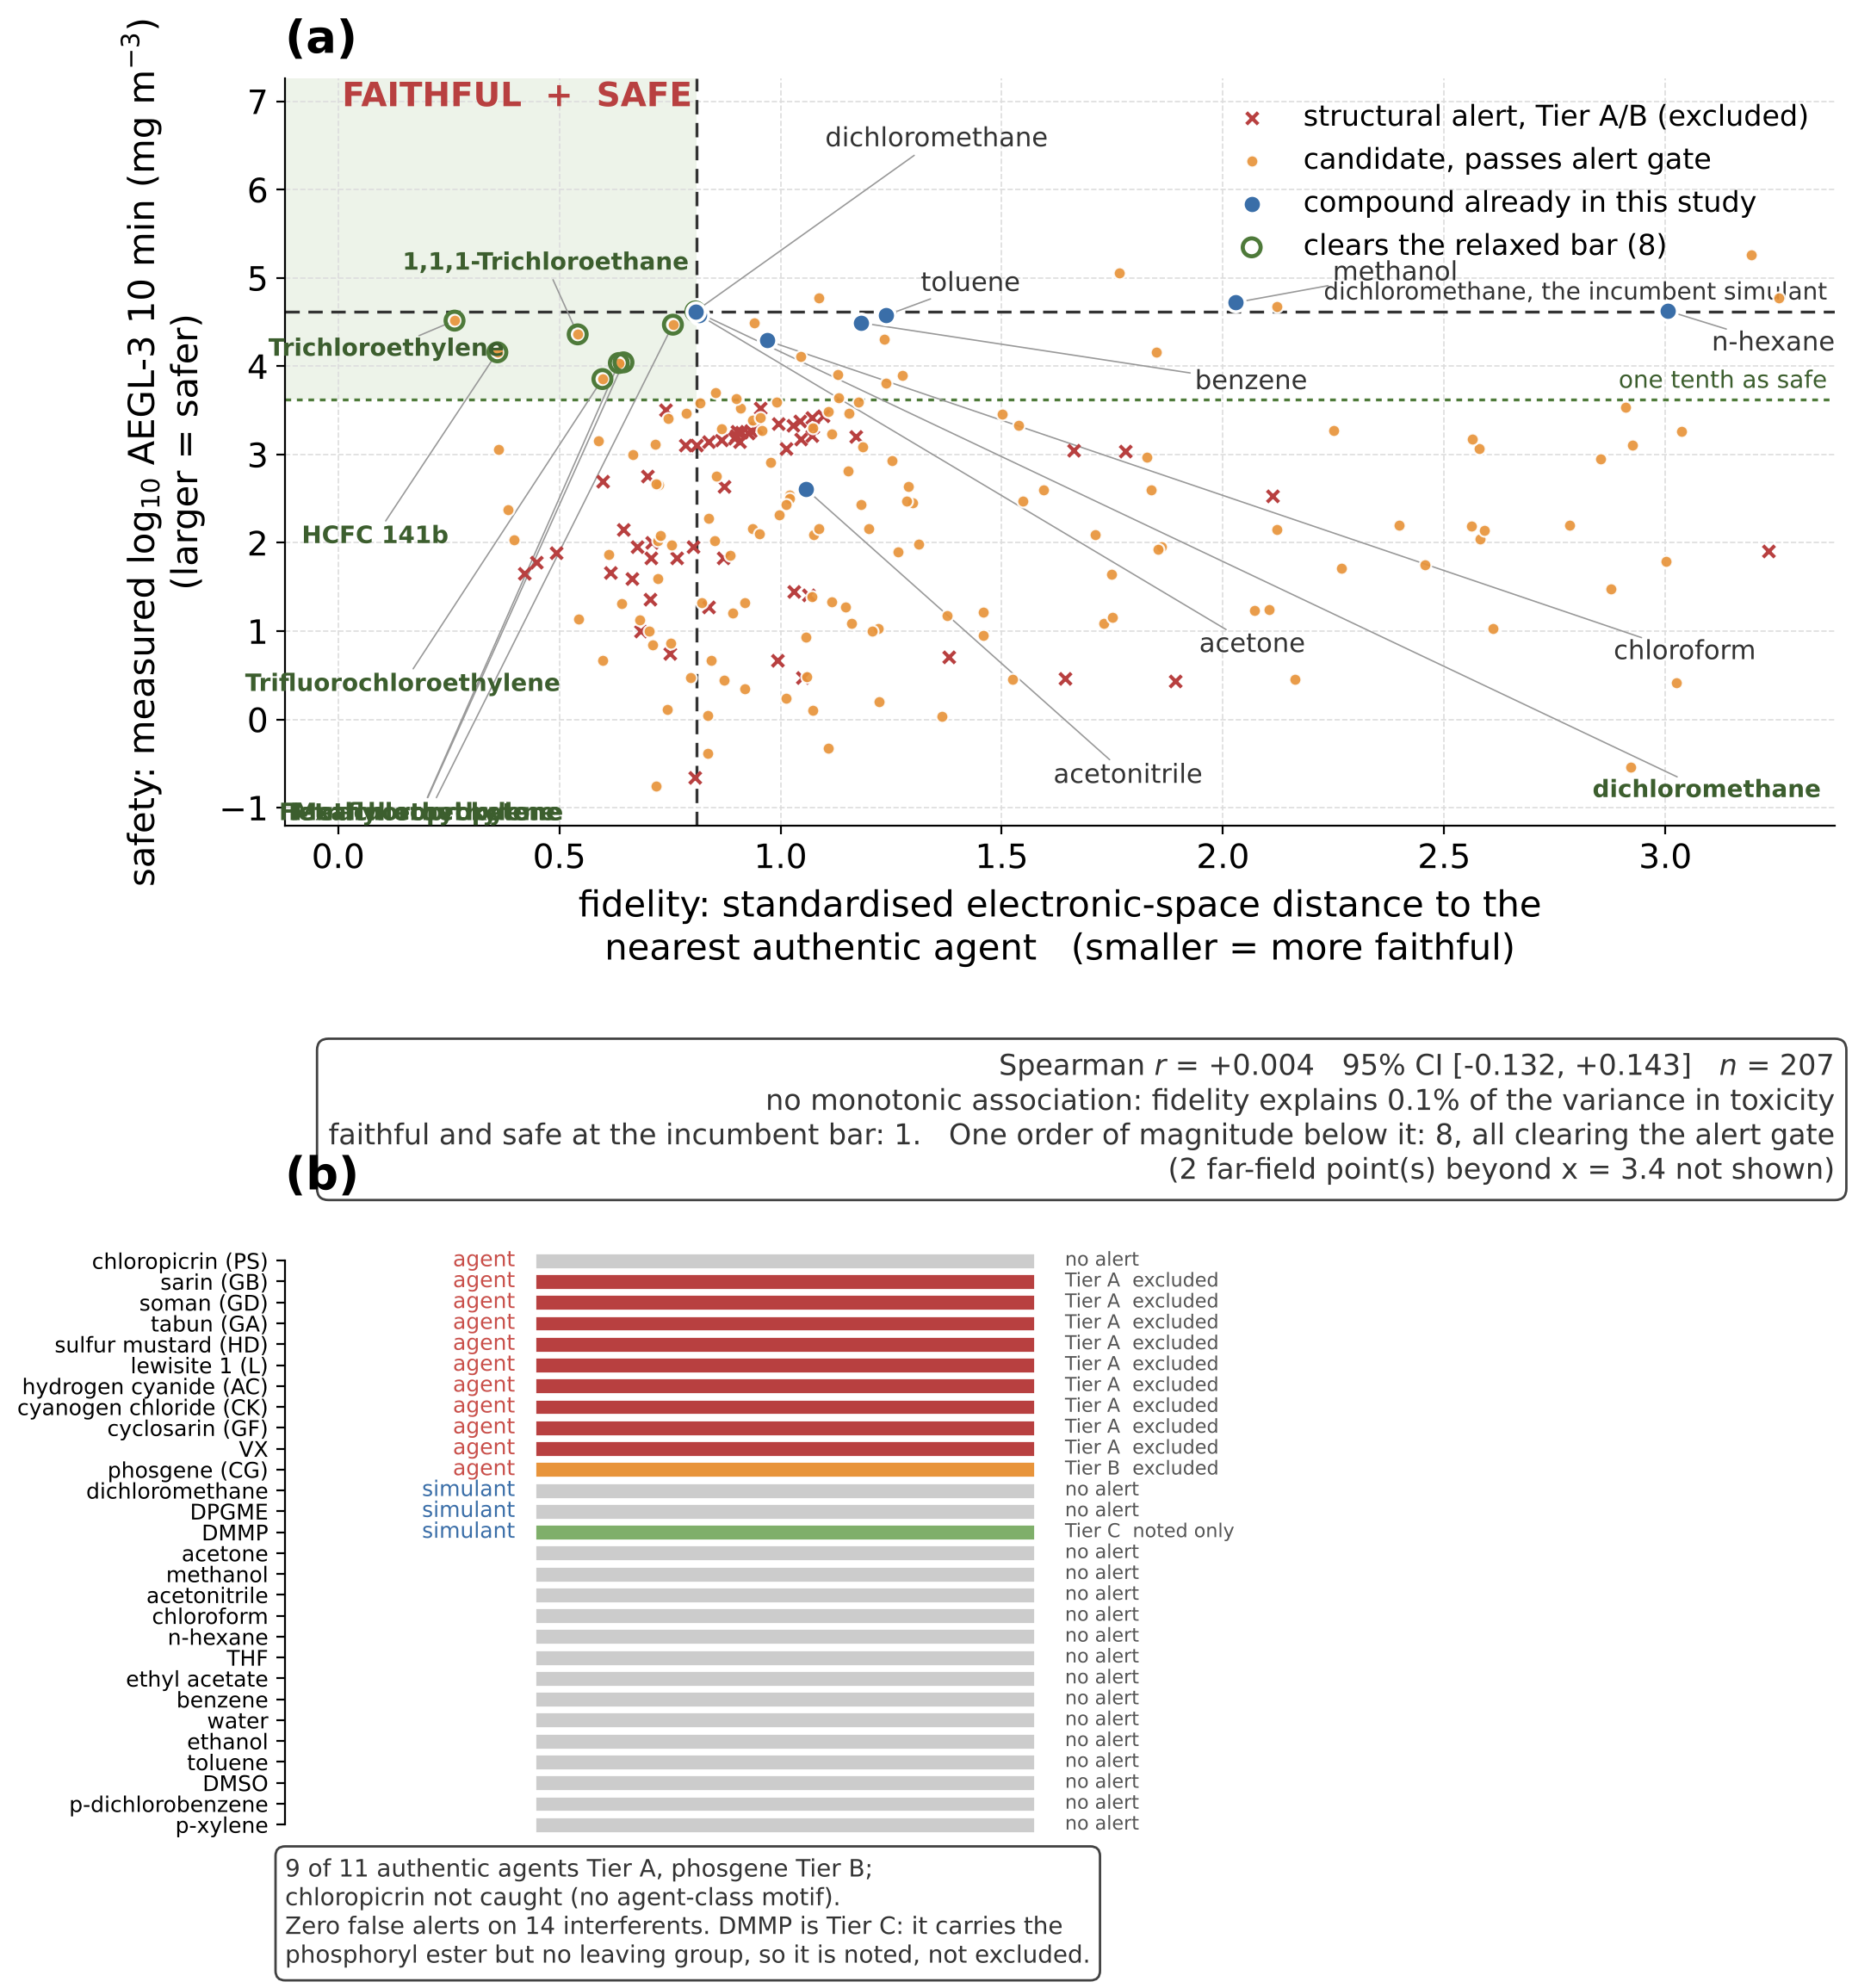
\includegraphics[width=\textwidth]{Fig_h1.png}
\caption{Fidelity and safety are not monotonically associated. (a) Electronic-space distance to
the nearest authentic agent against measured AEGL-3 for the 207 candidates
carrying both axes; crosses are compounds excluded by the structural filter. The
upper dashed line is the measured AEGL-3 of dichloromethane, the incumbent
simulant; the dotted line is one order of magnitude below it, and the eight
circled compounds are those that clear the lower bar while also falling in the
most faithful quartile.
(b) The filter applied to the twenty-eight-compound set: nine of eleven
authentic agents are Tier~A and phosgene Tier~B, there are no false alerts among
the interferents, and DMMP is Tier~C.}
\label{fig:h1}
\end{figure}

\subsection{Fidelity and safety are not monotonically associated}
\label{res:h1}

Across the 207 candidates carrying both measured axes (Fig.~\ref{fig:h1}a),
fidelity and safety are uncorrelated: Spearman $r=+0.004$ (95\% CI $-0.132$ to
$+0.143$), Pearson $r=-0.025$ (95\% CI $-0.177$ to $+0.133$, $p=0.73$), with
fidelity accounting for 0.06\% of the variance in toxicity
(Table~\ref{tab:h1}). The Spearman interval rules out any monotone association
stronger than $|r|=0.143$ and the Pearson interval any linear association
stronger than $|r|=0.177$, so this is a bounded negative result rather than an
underpowered one. Resembling an agent electronically does not require being as
dangerous as one.

\begin{table}[!htb]
\centering
\caption{Decoupling test. Fidelity is the standardised electronic-space distance to
the nearest authentic agent; safety is the measured EPA AEGL-3 (10~min).}
\label{tab:h1}
\small
\begin{tabular}{lc}
\hline
Quantity & Value \\
\hline
Candidates with both axes measured & 207 \\
Spearman $r$ & $+0.004$ (95\% CI $-0.132$ to $+0.143$) \\
Pearson $r$ & $-0.025$ (95\% CI $-0.177$ to $+0.133$), $p = 0.73$ \\
Variance of toxicity explained by fidelity & 0.06\% \\
\hline
Safety bar: dichloromethane, 41,685~mg~m$^{-3}$ & $\log_{10} = 4.62$ \\
Faithful and safe at that bar & 1 (the incumbent itself) \\
Faithful and safe one order of magnitude below it & 8 \\
\quad clearing the structural-alert gate & 8 \\
\quad more faithful than dichloromethane itself & 7 \\
Most faithful of them & Trichloroethylene (0.26 vs 0.81) \\
\hline
\end{tabular}
\end{table}

Setting the safety bar at the incumbent simulant's own measured value empties the
faithful-and-safe quadrant of everything but the incumbent: of the 207, the only
compound combining top-quartile fidelity with an AEGL-3 at or above
dichloromethane's 41\,685~mg~m$^{-3}$ is dichloromethane. That is a statement
about how safe dichloromethane is, not about how scarce candidates are. Seven
compounds in the whole pool exceed it on the safety axis and not one of them is
faithful.

Lowering the bar by one order of magnitude, to 4168~mg~m$^{-3}$, changes the
answer. Eight compounds then combine top-quartile fidelity with that level of
measured acute inhalation safety, every one of them clears the structural-alert
gate, and every one of them is more faithful than dichloromethane itself. In
order of fidelity they are trichloroethylene (0.26), HCFC~141b (0.36),
1,1,1-trichloroethane (0.54), trifluorochloroethylene (0.60),
tetrachloroethylene (0.63), hexafluoropropylene (0.64) and methyl ethyl ketone
(0.76), with dichloromethane itself (0.81) the eighth. The best of them,
trichloroethylene, is 3.1 times closer to the nearest authentic agent in the
electronic space while being only 1.3 times more acutely toxic by inhalation. At
two orders of magnitude below the incumbent the count rises to sixteen, all of
which clear the gate.

\begin{sloppypar}
These are candidates on the axes measured here, and that qualification is not a
formality. Trichloroethylene and tetrachloroethylene carry serious chronic and
carcinogenic hazard that an acute inhalation criterion does not express, and the
chlorofluorocarbons among them raise questions of atmospheric persistence rather
than of laboratory safety. What the screen establishes is narrower and still
useful: in the electronic space, compounds more faithful than the incumbent
exist at comparable acute inhalation safety, and they were not found by relaxing
the chemistry but by looking in the right descriptor space.
\end{sloppypar}

One limitation bounds this part of the result. The candidate pool is the set of
chemicals for which AEGL values exist, and chemicals receive AEGLs because they
are hazardous. Ordinary safe solvents are largely absent from the pool by
construction, which depresses the count at any bar. The seven compounds that
exceed dichloromethane on the safety axis illustrate the point from the other
side: two are hydrocarbon gases, one a refrigerant, one a monomer, and the three
a laboratory might actually reach for sit far out on the unfaithful side of the
electronic axis, well outside the top quartile that defines a faithful
candidate.

\subsection{The structural filter}

Applied to the 28-compound set (Fig.~\ref{fig:h1}b), the filter assigns Tier~A to nine of the eleven
authentic agents and Tier~B to phosgene, catching ten of eleven; chloropicrin
carries no agent-class motif and is not caught. There are no false alerts among
the fourteen interferents. DMMP is Tier~C: it carries the phosphoryl ester but
not a leaving group, which is precisely why it is used as a simulant and why it
is noted rather than excluded. Dichloromethane and DPGME raise no alert.


\section{Further discussion of the toxicity axis}
\label{S-disc}

The decoupling result is what makes the rest actionable. Because fidelity and
acute toxicity show no monotonic association across the compounds where both are
measured, the
pursuit of a simulant that is both faithful and safe is not a pursuit along a
trade-off curve, and the screen bears that out. Against the incumbent's own
safety value the quadrant is empty, which says more about dichloromethane than
about the chemistry: it is safer than all but seven of the 207 compounds in the
pool. One order of magnitude below that bar there are eight candidates, all of
them clearing the structural-alert gate and all of them more faithful than the
incumbent, with trichloroethylene 3.1 times closer to the nearest agent in the
electronic space at 1.3 times the acute inhalation toxicity.

We are not proposing trichloroethylene as a simulant. It carries chronic and
carcinogenic hazard that the axis used here does not express, and a replacement
chosen on two measured axes still has to survive the others. The claim is
narrower and, we think, more useful: the field's incumbent choice is not on the
efficient frontier of the two axes it is usually defended on, and better points
on those axes are already present among compounds with measured toxicity. That
the pool consists of chemicals assessed because they are hazardous depresses
every count reported here, so the seven are a lower bound rather than an
inventory. The constructive reading is that designing candidates and then
measuring them remains worthwhile, and that the filter excluding agent-class
motifs by construction can be applied from the start.

\paragraph{Limitations specific to this material.} The safety axis is acute inhalation lethality at
ten minutes and does not represent chronic, dermal or ocular hazard, nor
flammability, reactivity or environmental persistence, which is the main reason
the eight candidates of Section~\ref{res:h1} are presented as positions on two
axes rather than as recommendations. Four phosphorus-local descriptors exist for
six compounds only and are reported without being used in any 28-compound
analysis. Two features of the regulatory source are carried into our numbers and
should be read with them. Five of the nineteen panel values, and nine of the 259
in the wider set, are the agency's footnote values for exposures above half the
lower explosive limit; they are the agency's ten-minute AEGL-3 for those
compounds, but at concentrations where explosion rather than toxicity is the
governing hazard, which is a constraint on using them as working exposure
limits even though it does not affect their use here as a relative toxicity
scale. And the panel's p-xylene is matched to the compiled table's
\textit{Xylenes} entry (CAS 1330-20-7), which covers the mixed isomers rather
than the para isomer specifically; p-xylene's descriptors are its own, but its
safety-axis value is a class value.

\bibliography{refs}

\end{document}
